% ---- Writer 3 shared definitions also used here ----
\tikzset{
  w3box/.style={draw,rounded corners=2pt,fill=gray!12,align=center,font=\footnotesize,minimum height=8mm,inner sep=3pt},
  w3dark/.style={draw,rounded corners=2pt,fill=gray!30,align=center,font=\footnotesize,minimum height=8mm,inner sep=3pt},
  w3store/.style={draw,fill=white,align=center,font=\footnotesize,minimum height=8mm,inner sep=3pt,double,double distance=1pt},
  w3io/.style={draw,rounded corners=6pt,fill=white,align=center,font=\footnotesize,minimum height=8mm,inner sep=3pt},
  w3dec/.style={draw,diamond,aspect=2.2,fill=white,align=center,font=\scriptsize,inner sep=1pt},
  w3arr/.style={-{Stealth[length=2.2mm]},thick},
  w3dash/.style={-{Stealth[length=2.2mm]},thick,dashed},
  w3group/.style={draw,dashed,rounded corners=4pt,inner sep=5pt},
  w3lab/.style={font=\scriptsize,inner sep=1.5pt}
}

\subsection{Style extraction and handwriting synthesis}
\label{sec:styleprofile}
\label{sec:synthesis}

This subsection describes how a writer's style is learned from photographs of that writer's pages, stored permanently as a per-writer glyph library and set of style statistics, and later re-assembled into new text (functional units FU~2.5 to FU~2.7; requirements R1, R3, R6), component by component: cutting a joined line into characters, recovering an ordered pen path for each, filtering and summarising the result into a style profile, and finally the synthesiser that re-assembles profiles into new handwriting with a best-of-$N$ search.

Training a writer trains no network: a \emph{style profile} is one JavaScript Object Notation (JSON) file built once per writer, holding a library of that writer's own letter shapes (\emph{glyphs}, each a thin centre-line pen path) plus measured slant, letter height, spacing and joining statistics, after which no page images and no networks are needed to write in that style. The builder is an offline program using the recogniser of Section~\ref{sec:textrec} for inference only, run on ten pages each of the eight database writers (last labelled page held out) and the photographed pages of the five personal writers, 15\,\% of lines held out.

\subsubsection{Forced alignment: cutting a joined line into characters}
\label{sec:sty-forced}

In joined handwriting a character has no visible boundary, and no per-character labels exist, so the position of each letter has to be inferred from the line's own transcript and a recogniser that reads lines. \emph{Forced alignment} is the name for using a trained recogniser backwards: normally it is asked what the line says; here the answer is already known, and it is instead asked \emph{where} it saw each character of that known answer. Where the CTC training loss \emph{sums} the probability over every possible alignment, because for training it does not matter which was right, forced alignment takes the \emph{maximum} instead and keeps only the single most probable path, because here the alignment is precisely what is wanted. This is the Viterbi algorithm~\cite{viterbi1967}.

With the transcript's blank-augmented form $y'$ of length $S=2U+1$ and $\ell_t(k)=\ln y_t^k$ the recogniser's log-probabilities, $\delta_t(s)$ is the log-probability of the best path reaching position $s$ at step $t$:
\begin{equation}
\begin{split}
&\delta_1(1)=\ell_1(\varnothing),\quad\delta_1(2)=\ell_1(y'_2),\quad\delta_1(s)=-\infty\ (s>2),\\
&\delta_t(s)=\ell_t(y'_s)+\max\bigl\{\delta_{t-1}(s),\ \delta_{t-1}(s-1),\ \delta^{\mathrm{skip}}_{t-1}(s)\bigr\}.
\end{split}
\label{eq:sty-viterbi}
\end{equation}
where $\delta_t(s)$ is the log-probability of the best path reaching position $s$ of $y'$ at step $t$, $\varnothing$ is the blank symbol and $\delta^{\mathrm{skip}}_{t-1}(s)$ is the transition that jumps a blank between two distinct characters. Equation~\ref{eq:sty-viterbi} differs from the CTC sum of Equation~\ref{eq:rec-ctcprob} in one respect only: it maximises where the loss sums, because the alignment itself is wanted here rather than the total probability of the transcription. A back-pointer $\psi_t(s)$ is stored alongside every maximisation so the best path can be recovered once the recursion reaches $t=T$. Algorithm~\ref{alg:sty-viterbi} is this recursion stated as a procedure.

\begin{algorithm}[!htbp]
\caption{Forced alignment by Viterbi recursion (per time step $t$)}
\label{alg:sty-viterbi}
\begin{algorithmic}[1]
\REQUIRE blank-augmented transcript $y'$ of length $S$; log-probabilities $\ell_t(k)$, $t=1,\ldots,T$
\IF{$t=1$}
    \STATE $\delta_1(1)\leftarrow\ell_1(\varnothing)$; \ $\delta_1(2)\leftarrow\ell_1(y'_2)$; \ $\delta_1(s)\leftarrow-\infty$ for $s>2$
\ELSE
    \FOR{$s=1$ \TO $S$}
        \STATE candidates $\leftarrow\{\delta_{t-1}(s),\ \delta_{t-1}(s-1),\ \delta^{\mathrm{skip}}_{t-1}(s)\}$ \COMMENT{the skip term fires only where $y'$ allows it}
        \STATE $\delta_t(s)\leftarrow\ell_t(y'_s)+\max(\text{candidates})$; \ $\psi_t(s)\leftarrow\arg\max(\text{candidates})$
    \ENDFOR
\ENDIF
\IF{$t=T$}
    \STATE follow $\psi$ back from $\arg\max_s\delta_T(s)$ to recover the single best path \COMMENT{cost $O(TS)$ in total}
\ENDIF
\end{algorithmic}
\end{algorithm}

Back-pointers recovered from the maximisations give the whole best path at cost $O(TS)$. A CTC network emits a character at any single step inside its true extent, so the recovered span's \emph{centre} $c_k$ is reliable but its edges are not; the provisional boundary between two characters is the midpoint $\hat x_k=\tfrac12(c_{k-1}+c_k)$, refined to the cheapest nearby column by Equation~\ref{eq:sty-cut}, using that the only place a joined letter honestly ends is a ligature, which is both \emph{thin} (little ink in its column) and \emph{low} (near the baseline):
\begin{equation}
\begin{aligned}
\mathrm{cost}(x)&=\mathrm{thin}(x)+1.15\,\mathrm{top}(x),\qquad r=\max\bigl(3,\mathrm{round}(0.5x_h)\bigr),\\
x^*&=\arg\min_{|x-\hat x_k|\le r}\Bigl[\mathrm{cost}(x)+0.6\,\frac{|x-\hat x_k|}{r}\Bigr].
\end{aligned}
\label{eq:sty-cut}
\end{equation}

A line is dropped before its letters enter the library when its mean alignment log-probability falls below the 25th percentile of that same writer's own lines, a per-writer rather than absolute threshold, since the most difficult hands would otherwise lose almost everything; this discards 22 of 88 lines for writer 153. Cuts are forced strictly increasing within one line, since snapping each boundary independently can collapse two neighbours onto the same column.

The cuts are vertical rather than along the writer's slant, a measured design decision: glyphs cut along the slant carry a sheared edge that only matches their original neighbour and do not retile cleanly at new spacings, which lowered writer identification of synthesised output from 81.8\,\% to 68.6\,\% in a design-stage probe, so vertical cuts were kept, although no raw log of that probe survives.

\begin{figure}[htb]
\centering
\fbox{\parbox[c][4.5cm]{0.85\linewidth}{\centering [PLACEHOLDER --- one disconnected personal line and one strongly cursive line, with the aligned character centres and final ligature cuts marked as vertical lines on the ink]}}
\captionsetup{singlelinecheck=false,justification=justified}
\caption{Placeholder: forced-alignment cutting on a lightly connected hand and a strongly cursive hand side by side, showing the cuts land cleanly between letters on the first and are forced through genuine strokes on the second, which is why cursive hands are reproduced least legibly (Section~\ref{sec:syn-limits}).}
\label{fig:sty-cuts-fig}
\end{figure}


Algorithm~\ref{alg:sty-align} states the two routines that locate each character. The first is Equation~\ref{eq:sty-viterbi}: it differs from the CTC loss of Equation~\ref{eq:rec-alpha} in taking the \emph{maximum} where the loss takes a sum, which is what turns a probability into a single best alignment, and it keeps back-pointers so that the path itself can be recovered. The second is the cut cost of Equation~\ref{eq:sty-cut} evaluated for every column, which is minimised near the boundary to place the cut at a ligature --- that is, at a column that is both thin and low.

\begin{algorithm}[!htbp]
\caption{Forced alignment, and the per-column cut cost that places the boundary}
\label{alg:sty-align}
\begin{algorithmic}[1]
\STATE \textbf{ForcedAlign}(log-probabilities, transcript):
\STATE \quad build $y'\leftarrow$ blank-interleaved transcript \COMMENT{$S=2U+1$}
\STATE \quad $\delta[1,\cdot]\leftarrow-\infty$ except the first two positions
\FOR{$t=2$ \TO $T$}
    \FOR{every position $s$ simultaneously}
        \STATE $\mathrm{stay}\leftarrow\delta[t-1,s]$; \ $\mathrm{advance}\leftarrow\delta[t-1,s-1]$; \ $\mathrm{skip}\leftarrow\delta[t-1,s-2]$
        \IF{$y'_s$ is blank \OR $y'_s=y'_{s-2}$}
            \STATE $\mathrm{skip}\leftarrow-\infty$
        \ENDIF
        \STATE $\mathrm{best}\leftarrow$ the largest of the three \COMMENT{\textbf{maximum}, not a sum: this is the one change from Algorithm~\ref{alg:rec-ctc}}
        \STATE $\mathrm{backpointer}[t,s]\leftarrow$ which one won
        \STATE $\delta[t,s]\leftarrow\mathrm{best}+\log\mathrm{Prob}[t,y'_s]$
    \ENDFOR
\ENDFOR
\STATE \quad back-trace from the better of the last two positions
\STATE \quad character $i$ owns the frames whose winning position is $2i$
\STATE
\STATE \textbf{CutCostPerColumn}(column ink profile, baseline, x-height):
\STATE \quad $\mathrm{smoothed}\leftarrow$ profile averaged over $\max(3,\mathrm{round}(0.12\,x_h))$ columns, odd
\STATE \quad $\mathrm{thin}\leftarrow\mathrm{smoothed}\,/\,$ 60th percentile of the non-empty columns
\STATE \quad $\mathrm{topAbove}\leftarrow(\text{baseline}-\text{highest ink row})/x_h$, clipped to $[0,3]$
\STATE \quad $\mathrm{cost}\leftarrow\mathrm{thin}+1.15\,\mathrm{topAbove}$
\STATE \quad $\mathrm{cost}\leftarrow0$ wherever the column holds no ink \COMMENT{a true gap is free}
\end{algorithmic}
\end{algorithm}

\subsubsection{From ink to ordered pen paths}
\label{sec:sty-trace}

A thinned image is a picture of the pen's path, not yet an \emph{ordered} path, and four geometric operations recover the ordering, each resting on the 8-neighbourhood degree of a skeleton pixel: degree one is a stroke end, two an interior point, three or more a junction. The skeleton is \emph{traced} into chains grown from each unvisited end or junction, stopping at a junction rather than choosing a branch there, which is what makes the decomposition unique --- a junction being precisely the point where the true pen order cannot be recovered from the image alone. Short false branches left by thinning are \emph{pruned} as spurs; because a self-crossing stroke such as the loop of an e breaks into several chains at the crossing although the pen never lifted, nearby chain ends with nearly opposed directions are \emph{re-joined}; and each chain is finally \emph{simplified} by the Douglas--Peucker recursion~\cite{douglas1973} at $\varepsilon=0.6$ pixels.

The line is binarised and thinned by the same functions as Section~\ref{sec:wid-strokenorm} (Otsu, rule removal, closing, Zhang--Suen~\cite{zhang1984}), with the \emph{slant} scored on the ink's column histogram sheared by a trial angle $\theta$:
\begin{equation}
x'_i(\theta)=\bigl\lfloor x_i-(y_i-\bar y)\tan\theta\bigr\rfloor,\qquad H_\theta(c)=\#\{i:x'_i(\theta)=c\},\qquad \hat\theta=-\arg\max_\theta\sum_cH_\theta(c)^2 .
\label{eq:sty-slant}
\end{equation}
where $(x_i,y_i)$ are the ink coordinates, $\bar y$ the mean ink row, $x'_i(\theta)$ the column each pixel falls into after shearing by a trial angle $\theta$, $H_\theta$ the resulting column histogram and $\hat\theta$ the estimated slant. Equation~\ref{eq:sty-slant} maximises the sum of squared bin counts for the same reason as the deskew objective of Equation~\ref{eq:seg-skew}: shearing conserves the total ink, so the sum of squares is largest when vertical strokes stack into the fewest columns, which happens when the shear has cancelled the writer's slant.

Each simplified point of a chain in territory $[L,R)$ is then mapped by Equation~\ref{eq:sty-norm} into a writer-independent frame, baseline 0, unit x-height, slant removed, the same normalisation goal pursued for cursive word images in the literature~\cite{vinciarelli2001}:
\begin{equation}
y_n=\frac{y_b-y}{x_h},\qquad x_n=\frac{x-L}{x_h}-\sigma\,y_n,\qquad\sigma=\tan\hat\theta .
\label{eq:sty-norm}
\end{equation}

The whole line is thinned \emph{once}, before territory cuts are applied to the traced centre lines, because thinning each slice separately would create a spurious spine along the cut boundary. On a side confirmed connected, the outward-running low connector is trimmed when enough of the glyph width survives, and the entry and exit heights are recorded for the synthesiser's own connector (Section~\ref{sec:syn-place}).


Thinning leaves a one-pixel-wide set of ink pixels, which is a picture of the pen path and not yet an ordered path.
Four operations recover the ordering, and each rests on the 8-neighbourhood degree of a skeleton pixel $p$,
\begin{equation}
\deg(p)=\#\bigl\{q\in\mathcal N_8(p)\ :\ q\ \text{is a skeleton pixel}\bigr\},
\label{eq:app-degree}
\end{equation}
which classifies every pixel by Equation~\ref{eq:app-degree}: an \emph{end} has $\deg=1$, an \emph{interior} pixel $\deg=2$, and a \emph{junction} $\deg\ge3$.

\emph{Tracing.}
A chain is grown from each unvisited end or junction and extended through interior pixels only, stopping at the next end or junction, so that the chain set covers every skeleton pixel exactly once and each chain is an ordered pixel sequence.
Stopping at junctions rather than choosing a branch there is what makes the decomposition unique: a junction is a point at which the true pen order is not recoverable from the image, so the decision is deferred to the re-joining rule below rather than taken arbitrarily.

\emph{Spur pruning.}
Thinning a stroke of finite width leaves short false branches at the ends of real strokes.
A chain is discarded as a spur when
\begin{equation}
\mathrm{len}(C)<2.5\ \text{pixels}\quad\wedge\quad \exists\,p\in\{p_1,p_{|C|}\}\ :\ \deg(p)=1,
\label{eq:app-spur}
\end{equation}
that is when it is shorter than 2.5 pixels \emph{and} has at least one free end.
The conjunction in Equation~\ref{eq:app-spur} matters: a short chain between two junctions is the crossbar of a letter such as A or the waist of an e and must be kept, whereas a short chain hanging off a junction carries no pen motion.

\emph{Junction re-joining.}
A self-crossing stroke, such as the loop of an e or the ascender of an l, breaks into several chains at the junction where it crosses itself, although the pen never left the paper.
Two chain ends $i$ and $j$ are re-joined into one chain when they are close and nearly collinear,
\begin{equation}
\lVert p_i-p_j\rVert\le1.5\ \text{pixels}\quad\wedge\quad \arccos\bigl(-\mathbf d_i\cdot\mathbf d_j\bigr)<75^\circ,
\label{eq:app-rejoin}
\end{equation}
where $\mathbf d_i$ and $\mathbf d_j$ are the unit outward directions of the two chains at those ends.
The negative sign in Equation~\ref{eq:app-rejoin} is the continuation test rather than a parallelism test: two chains continue each other when one runs \emph{into} the junction along the direction the other runs \emph{out} of it, so their outward directions are nearly opposed and $-\mathbf d_i\cdot\mathbf d_j$ is near $+1$.
A threshold of $75^\circ$ admits the curvature a pen shows through a crossing while rejecting a genuine corner, at which the two strokes meet at nearer a right angle.

\emph{Curve simplification.}
A traced chain holds one point per pixel, far more than a pen path needs, and its points lie on a lattice.
Each chain is therefore simplified by the Douglas--Peucker recursion~\cite{teikari2016}: for a chain from $p_1$ to $p_n$, the vertex of greatest perpendicular distance from the straight line joining its ends,
\begin{equation}
d_{\max}=\max_{1<i<n}\frac{\bigl\lvert(p_n-p_1)\times(p_i-p_1)\bigr\rvert}{\lVert p_n-p_1\rVert},
\label{eq:app-dp}
\end{equation}
is found; if $d_{\max}\le\varepsilon$ the whole chain is replaced by its two end points, and otherwise it is split at that vertex and both halves simplified in the same way.
With $\varepsilon=0.6$ pixels, which is 0.05 to 0.12\,mm at 4\,mm per x-height, the deviation of the simplified path from the traced one is bounded by $\varepsilon$ everywhere by construction.
Equation~\ref{eq:app-dp} measures distance to the infinite line through the two ends, which fails on a closed chain: there the two ends coincide, the denominator vanishes and the whole loop would collapse to two points.
A chain whose ends lie within $\max\bigl(1.5,\,0.25\max_i\lVert p_i-p_0\rVert\bigr)$ pixels of each other is therefore split at its farthest vertex first and simplified in two open halves, which is what keeps the loops of e, l and o.

\emph{Resampling and smoothing.}
Thinning leaves a staircase on a diagonal stroke, whose median turn angle is $8.9^\circ$ with a 90th percentile of $59.5^\circ$; drawn directly, that staircase appears as tremor.
Kept variants are therefore resampled at 0.055 x-heights of arc length and smoothed by two passes of the three-point average
\begin{equation}
q_i\leftarrow\tfrac14q_{i-1}+\tfrac12q_i+\tfrac14q_{i+1},
\label{eq:app-smooth}
\end{equation}
with the end points held fixed.
Equation~\ref{eq:app-smooth} is a binomial kernel, so it attenuates the highest representable spatial frequency --- the alternating lattice staircase --- completely while leaving a smooth curve almost unchanged, and fixing the ends preserves the entry and exit points that the synthesiser's connectors attach to.

\subsubsection{Glyph quality gates and the cross-writer letter prior}
\label{sec:sty-gates}

Of about 2\,122 to 4\,031 raw instances per writer, roughly 10\,\% survive five gates, ordered cheapest-first and most-local-first: geometry, outliers, a cross-writer prior, consensus against the same writer's other instances of that letter, and typicality. The hardest to design is the cross-writer prior, because deciding whether a letter is malformed needs more examples of well-formed letters than one writer's ten pages contain; thirteen writers together do, so whatever all thirteen hands agree on is taken to be the letter itself rather than any one style.

Each glyph is reduced to a $12\times12$-grid shape descriptor $v_g$ (144 numbers), damped, blurred across neighbouring cells and scaled to unit length so pen thickness cancels. The reference shape $\bar v_c$ for character $c$ is the element-wise median over all thirteen writers, also unit length, and the prior distance is their cosine distance:
\begin{equation}
\mathrm{priorD}(g,c)=1-v_g\cdot\bar v_c\in[0,1],
\label{eq:sty-prior}
\end{equation}
with the 70\,\% of each writer's variants having the smallest $\mathrm{priorD}$ kept. Equation~\ref{eq:sty-prior} only ever \emph{rejects} one of the writer's own variants; it never substitutes a shape from another writer, so no other person's handwriting can enter a profile through this gate. What it measures is \emph{typicality}, not legibility, and a writer whose letters are consistently unusual scores badly on a prior built from everyone else.

Two further glyphs are derived per character: the \emph{medoid}, the one real variant with the smallest total $L_1$ distance to the character's other variants, used as the \emph{anchor} fallback of Section~\ref{sec:syn-glyph} because it is a real pen stroke rather than an average of several; and the \emph{denoised prototype}, the per-stroke median curve of the largest group of same-stroke-count variants, prepended only when clearly cleaner than the variants it summarises.

\begin{figure}[!htbp]
\centering
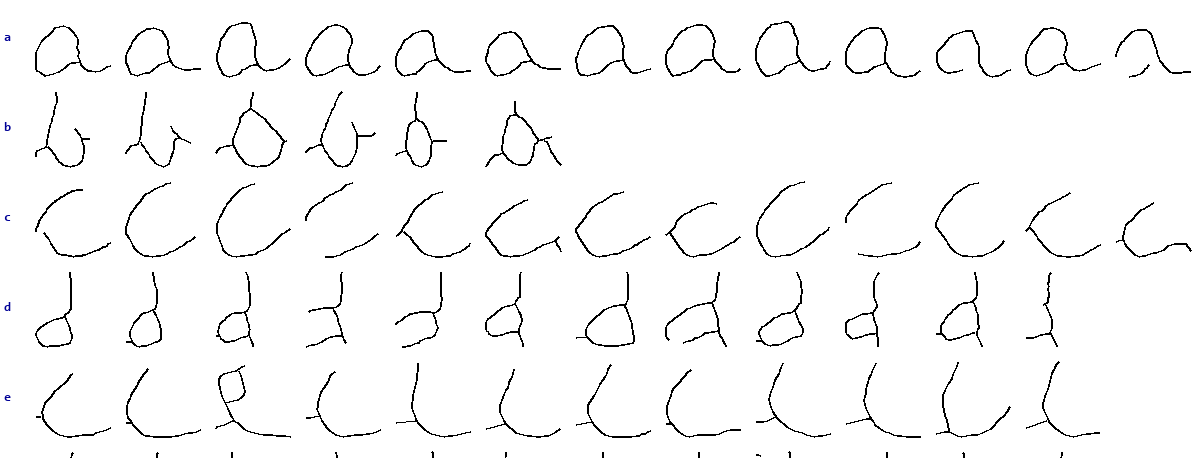
\includegraphics[width=0.78\linewidth]{Figures/w3_glyphs153_ae.png}
\caption{Stored variants of the letters a, b, c, d and e of writer 153, a strongly joined hand; each row is one character with up to 12 variants, the short tails at the sides being remains of ligatures.}
\label{fig:sty-glyphs}
\end{figure}



About 2\,122 to 4\,031 raw instances are extracted per writer and roughly \textbf{10\,\%} survive. Five gates are applied per character, in the order of Table~\ref{tab:sty-gates}. The cascade is ordered cheapest-first and most-local-first: the geometric tests reject on properties of \emph{one} glyph, the prior on agreement with \emph{all thirteen} writers, and the last two on agreement with \emph{that writer's own} other instances of the same letter, so a glyph is only compared with its peers once it is known to be a plausible letter at all.

\begin{table}[!htbp]
\centering
\fontsize{8}{9.6}\selectfont
\setlength{\tabcolsep}{3.5pt}
\renewcommand{\arraystretch}{1.05}
\begin{tabularx}{\linewidth}{|c|p{2.1cm}|X|p{2.3cm}|p{1.9cm}|}
\hline
\textbf{\#} & \textbf{Gate} & \textbf{Test} & \textbf{Compared against} & \textbf{Survivors} \\
\hline
1 & Geometry & Size limits, at most six strokes, a class prior on height, the absence of a swallowed neighbour, and a pen length above the adaptive floor $\max(0.30,\,0.5\,\tilde p_c)$ on that character's own median pen length $\tilde p_c$. The floor is adaptive because one fixed value either kept neighbour bleed or discarded genuinely short letters. & the glyph itself & \mustdo{\%} \\
\hline
2 & Outliers & Width and height must lie within fixed ratios of the 40th-percentile width and the median height. & that letter's own distribution & \mustdo{\%} \\
\hline
3 & Cross-writer prior & Keeps the \textbf{70\,\%} nearest the pooled shape, by Equation~\ref{eq:sty-prior}. & all thirteen writers & 70\,\% \\
\hline
4 & Consensus & Keeps the nearest \textbf{75\,\%} to the L1-medoid of the kept descriptors, which removes glyphs contaminated by a neighbour. & that writer's own instances & 75\,\% \\
\hline
5 & Typicality & Keeps the best \textbf{12} by closeness to the reference width and height. & that writer's own instances & $\le12$ \\
\hline
\multicolumn{4}{|r|}{\textbf{end to end, measured}} & \textbf{about 10\,\%} \\
\hline
\end{tabularx}
\caption{The five quality gates, in the order applied. Only the last three have a stated keep-fraction by construction; the first two reject a variable number, which is why the end-to-end survival rate is measured rather than predicted from the product of the gates.}
\label{tab:sty-gates}
\end{table}

\mustdo{record how many instances each of gates~1 and~2 rejects, over all thirteen writers, so that the \textbf{10\,\%} end-to-end figure can be resolved into the five gates rather than only measured at the end.}

\begin{figure}[htb]
\centering
\figmaybe{sty-gates-cascade.png}{width=0.85\linewidth}{A funnel or bar chart of instance counts surviving each of the five gates of Table~\ref{tab:sty-gates}, for one writer, from the raw extraction to the final twelve variants per character; and beside it a strip of eight instances of one letter, those rejected marked with which gate rejected them.}
\caption{Instances surviving each of the five quality gates for one writer, with examples of what each gate rejects.}
\label{fig:sty-gates}
\end{figure}


\subsubsection{Style statistics and permanent storage}
\label{sec:sty-stats}

Besides glyphs, the profile holds measured numbers: slant, pixel x-height, ascender and descender reach, word gap, and \emph{connectedness}, the fraction of adjacent letter pairs whose connection flag was set during tracing. Table~\ref{tab:sty-writers} shows the diversity this is built to reproduce --- slant $-10.5^\circ$ to $42.0^\circ$, connectedness 0.195 to 0.968, word gap 0.94 to 2.68 x-heights across the thirteen writers --- which is requirement R1's diversity target, and the thirteen files (about 4.8\,MB total) load when the server starts.

\begin{table}[!htbp]
\centering
\fontsize{7.5}{9}\selectfont
\setlength{\tabcolsep}{2.5pt}
\begin{tabular}{|l|r|r|r|r|r|r|r|}
\hline
\textbf{Writer} & \textbf{Lines} & \textbf{Slant ($^\circ$)} & \textbf{$x_h$ (px)} & \textbf{$A$} & \textbf{$D$} & \textbf{Gap} & \textbf{Conn.} \\
\hline
150 & 61 & $-4.5$ & 47 & 1.58 & $-0.72$ & 1.33 & 0.343 \\
151 & 58 & 33.0 & 22 & 2.69 & $-1.09$ & 1.59 & 0.968 \\
153 & 66 & 30.0 & 33 & 1.59 & $-1.10$ & 1.59 & 0.961 \\
384 & 54 & 4.5 & 43 & 1.93 & $-0.71$ & 1.37 & 0.500 \\
552 & 47 & $-10.5$ & 32 & 1.62 & $-0.56$ & 1.53 & 0.609 \\
dylan & 79 & $-6.0$ & 26 & 1.68 & $-0.62$ & 1.79 & 0.195 \\
thiya & 48 & 30.75 & 15 & 2.24 & $-1.00$ & 1.65 & 0.962 \\
yeukita & 74 & 0.0 & 27 & 1.45 & $-0.58$ & 0.94 & 0.417 \\
\hline
\end{tabular}
\caption{Representative rows of the thirteen stored style profiles (schema in Table~\ref{tab:sty-schema}): kept lines, slant, pixel x-height, ascender $A$, descender $D$, word gap in x-heights, and connectedness.}
\label{tab:sty-writers}
\end{table}

\begin{figure}[htb]
\centering
\fbox{\parbox[c][4cm]{0.75\linewidth}{\centering [PLACEHOLDER --- scatter or bar plot of connectedness vs.\ reproduced character accuracy across the thirteen writers]}}
\captionsetup{singlelinecheck=false,justification=justified}
\caption{Placeholder: connectedness (Table~\ref{tab:sty-writers}) plotted against each writer's reproduced character accuracy from Table~\ref{tab:syn-evid}, to show quantitatively that the most joined hands are the hardest to reproduce.}
\label{fig:sty-conn-fig}
\end{figure}

\mustdo{\emph{The builder's \texttt{ExtractLineGlyphs} currently raises an import error} (a stale reference to a function moved during the restructuring of \texttt{TrainText.py}), so no new writer can presently be added and none of the thirteen stored profiles can be regenerated from the page images; the stored profiles themselves are unaffected and still load correctly. \texttt{legibilityLambda} is also absent from all thirteen stored files, so the system synthesises every writer at $\lambda=0$ until the tuner is re-run (Section~\ref{sec:syn-limits}).}


A profile is one text file per writer, and Table~\ref{tab:sty-schema} lists the keys that carry design meaning, with the values of one writer as an example.

\begin{table}[!htbp]
\centering
\fontsize{7.5}{9}\selectfont
\setlength{\tabcolsep}{3pt}
\renewcommand{\arraystretch}{1.05}
\begin{tabularx}{\linewidth}{|p{2.6cm}|X|p{2.1cm}|}
\hline
\textbf{Key} & \textbf{Meaning} & \textbf{Example (153)} \\
\hline
\texttt{slantDeg}, \texttt{xHeightPx}, \texttt{strokeWidthXh} & Median slant (Equation~\ref{eq:sty-slant}), median pixel x-height and ink area divided by skeleton length in x-heights. & 30.0, 33.0, 0.189 \\
\hline
\texttt{ascender}, \texttt{descender} & Typical reach of tall and descending lower-case glyphs, in x-heights (defaults 1.7 and $-0.6$). & 1.59, $-1.10$ \\
\hline
\texttt{wordSpaceXh}, \texttt{connectedness} & Word gap measured on the real ink, in x-heights; fraction of adjacent in-word letter pairs that the pen joins. & 1.59, 0.961 \\
\hline
\texttt{letterAdvance} & Median advance of each character, in x-heights (45 keys). & \texttt{T}: 1.438, \texttt{e}: 1.147 \\
\hline
\texttt{slantMeasRef}, \texttt{ascMeasRef}, \texttt{descMeasRef} & Slant and reach of the real full lines, measured with the estimators later used on synthesised renders; input of the style calibration (Equation~\ref{eq:syn-cal}). & 30.0, 1.933, $-1.468$ \\
\hline
\texttt{glyphs}, \texttt{idealGlyphs}, \texttt{idealMedoid} & Variant library: per character up to 12 kept variants and a prepended prototype, each holding its \texttt{strokes} as $[x,y]$ points in x-heights (baseline $y=0$, upright) with the width, advance, lead, reach, entry and exit coordinates, connection flags and $\mathrm{priorD}$ the synthesiser needs; then the per-stroke median prototype and the medoid, which is the anchor. & 37 characters, 283 variants; 23 and 29 prototypes \\
\hline
\texttt{legibilityLambda} & Legibility parameter $\lambda$ of Equations~\ref{eq:syn-global} and~\ref{eq:syn-swap}; written by the tuner after the build, \emph{not} by the builder. \emph{Absent from all thirteen stored profiles}, so the deployed code falls back to $\lambda=0$. & not present \\
\hline
\end{tabularx}
\caption{Keys of a style-profile file (JavaScript Object Notation) that carry design meaning; bookkeeping keys and the grey-level reference statistics are omitted. The example column was re-read from the stored file \texttt{StyleProfiles10/153.json}. The whole library is geometry in x-height units, which is why one profile serves any pen size.}
\label{tab:sty-schema}
\end{table}

\subsubsection{Synthesis: choosing and placing a glyph}
\label{sec:syn-glyph}
\label{sec:syn-place}

The synthesiser takes text, a style profile, a pen size $x_{\mathrm{mm}}$ in millimetres and a random seed, and returns a \emph{trajectory}, pen-down polylines in millimetres; geometry stays in x-height units until one multiplication at the end, so one profile serves any pen size. Requirement R1 pulls in two directions at once: handwriting that resembles the writer argues for always using the writer's own letters, while handwriting that can be read argues for replacing the writer's worst letters with something clearer. The parameter $\lambda\in[0,1]$ is the single control that sets where a writer sits between those two. The obvious way to trade them off, blending the writer's glyph and a clear \emph{anchor} glyph geometrically, is \emph{not} used, because an average of two different pen strokes is usually not a valid letter at all; instead $\lambda$ scales the \emph{probability} that a chosen variant is replaced by the anchor outright, so every letter drawn is always a real letterform.

Global shear, join probability and line pitch follow from the profile (Equation~\ref{eq:syn-global}); among a writer's own variants for one character the choice is weighted by rank and, when joining, by how well the variant's entry height matches where the pen already is; the anchor-substitution probability is Equation~\ref{eq:syn-swap}; and placement is Equation~\ref{eq:syn-place-eq}:
\begin{align}
\theta_{\mathrm{cap}}&=45^\circ-19^\circ\lambda,\quad\sigma=\tan\!\bigl(\operatorname{clip}(\theta_{\mathrm p},\pm\theta_{\mathrm{cap}})\bigr)+\Delta_\sigma,\quad p_{\mathrm j}=\min(c,1),\label{eq:syn-global}\\
P_{\mathrm{swap}}(\lambda,d)&=\begin{cases}1&d\ge0.55,\\0&\lambda\le10^{-3},\\0.06\,\lambda&d\le0.12,\\\operatorname{clip}\bigl(\lambda\,(0.55+0.9\,b),0,1\bigr),\ b=\operatorname{clip}\bigl(\tfrac{d-0.12}{0.43},0,1\bigr)&\text{otherwise,}\end{cases}\label{eq:syn-swap}\\
X&=P_x+(\ell+x+\sigma_g\,y)\,x_{\mathrm{mm}},\qquad Y=P_y+(y+\delta_g)\,x_{\mathrm{mm}}.\label{eq:syn-place-eq}
\end{align}
A variant beyond prior distance $d=0.55$ is replaced \emph{unconditionally}, whatever $\lambda$; one closer than $d=0.12$ is kept almost always; between those the probability rises with both $d$ and $\lambda$. Below $\lambda=10^{-3}$ substitution switches off entirely, so a writer tuned to zero keeps even their marginal letters. When a writer's medoid itself is too malformed to serve as the anchor, a hand-designed single-stroke skeleton (joined cursive or upright print, re-proportioned to that writer's ascender and descender reach) is used instead, reading back at about 96\,\% character and 84\,\% word accuracy, which is what makes it a usable floor.

Treating connectedness $c$ as a hard threshold, joining every pair above it, was tried first and fused whole words into unbroken blobs, losing the irregularity that makes a hand look human; it is used as a per-pair \emph{probability} $p_{\mathrm j}$ instead. Measured over a design-stage probe, the anchor share this produces ran from 0\,\% for writer 552 to 76\,\% for writer 151, the most joined hand of the set. One pseudo-random stream seeded by the seed argument supplies every draw, so the arguments fix the output completely; at the jitter amplitude the search uses, a letter is perturbed by about a $1.1^\circ$ rotation, a 2.5\,\% scale change and under 0.05\,mm translation. \emph{Style calibration}: because glyphs are placed one instance at a time, an assembled line does not automatically reproduce the writer's own line-level slant and ascender reach (writer 150's ascenders came out about 7\,\% too tall, writer 551's slant about $9^\circ$ too steep against real lines), so a fixed probe sentence is synthesised once per writer and three fixed-point iterations of Equation~\ref{eq:syn-cal} adjust the shear shift $\Delta_\sigma$ and the scale factors $K_A$, $K_D$ until the probe matches the stored real-line reference values:
\begin{equation}
\Delta_\sigma\leftarrow\Delta_\sigma+\tan\theta_{\mathrm{ref}}-\tan\theta_{\mathrm{got}},\quad K_A\leftarrow\operatorname{clip}\Bigl(K_A\frac{A_{\mathrm{ref}}-1}{A_{\mathrm{got}}-1},0.5,1.6\Bigr),\quad K_D\leftarrow\operatorname{clip}\Bigl(K_D\frac{D_{\mathrm{ref}}}{D_{\mathrm{got}}},0.5,1.6\Bigr),
\label{eq:syn-cal}
\end{equation}
with ``ref'' the stored real-line value and ``got'' the probe's measured value by the estimators of Section~\ref{sec:sty-trace}, each correction clipped to bound its effect.

\begin{figure}[htb]
\centering
\fbox{\parbox[c][4.5cm]{0.85\linewidth}{\centering [PLACEHOLDER --- the same letter drawn at $\lambda=0$, $\lambda=0.5$ and $\lambda=1$ for one strongly joined writer, each candidate's prior distance $d$ and swap probability printed beside it]}}
\captionsetup{singlelinecheck=false,justification=justified}
\caption{Placeholder: the legibility sweep of Equation~\ref{eq:syn-swap} on one writer's worst-scoring letter, from the writer's own glyph through partial anchor substitution to the full anchor, with $P_{\mathrm{swap}}$ plotted against prior distance $d$ for several $\lambda$ as an inset curve.}
\label{fig:syn-swap-fig}
\end{figure}


Every constant of the glyph choice, the placement, the joins and the randomness is listed in Table~\ref{tab:syn-const} with the design reason for its value, so that Section~\ref{sec:synthesis} can describe the construction without interrupting it to justify a number.

\begin{table}[!htbp]
\centering
\fontsize{8}{9.6}\selectfont
\setlength{\tabcolsep}{4pt}
\begin{tabularx}{\linewidth}{|p{3.5cm}|p{3.2cm}|X|}
\hline
\textbf{Constant} & \textbf{Value} & \textbf{Reason for the value} \\
\hline
Eligible variants per letter & 5 best by $\mathrm{priorD}$ & 80.5 against 75.5\,\% writer identification over all twelve \\
Anchor taken from the medoid & $\mathrm{priorD}\le0.30$ & above it, not clean enough; skeleton used instead \\
Cursive anchor threshold & $c\ge0.5$, off above 1 & 0.3 lowered the evaluation score \\
Anchor re-proportioning & $y\mapsto1+(y-1)\max(0.35,\frac{A-1}{0.75})$, $y\mapsto y\max(0.35,\frac{|D|}{0.55})$ & skeleton takes the writer's reach; floor 0.35 keeps it from flattening \\
Pen advance & the glyph's own advance & never the character median \\
Anchor shear cap & $\pm\tan30^\circ$, $\pm\tan22^\circ$ print & $40^\circ$ collides even for a clean letter \\
Collision guard & $0.05\,x_{\mathrm{mm}}$ & shift right rather than let ink touch \\
Word gap & $g\,x_{\mathrm{mm}}(0.85+0.3u)$, $u\sim U(0,1)$ & so words do not fall on a grid \\
Line width; pitch & 185\,mm in the server; $L$ (Eq.~\ref{eq:syn-global}) & wrap inside the work area; writer's line spacing \\
Connector sag & $\min(0.11x_{\mathrm{mm}},0.16|\Delta x|)$, plus noise & span-proportional: a fixed dip loops a short join \\
Polyline resampling & 0.35\,mm of arc length & even plotter motion \\
Jitter rotation; scale; translation & $2.2^\circ J$; $0.05J$; $0.022J$ and $0.0132J$ x-heights & one amplitude sets how unsteady the hand looks \\
Jitter amplitude $J$ & 0.15 default, 0.5 search, 0.15 anchors & the search needs spread; anchors exist to stay legible \\
Baseline drift & walk of $0.05J\cdot0.35$ per glyph, clipped $\pm0.25$ x-heights & wanders slowly, clipped to stay on the line \\
Judges' render settings & 0.085 x-height pen, blur 0.30 of it, 18 px/mm, pad $0.18\,x_{\mathrm{mm}}$ & identical ink for every candidate (Section~\ref{sec:syn-search}) \\
\hline
\end{tabularx}
\caption{Constants of the synthesiser, with the design reason for each. Lengths in $x_{\mathrm{mm}}$ scale with the pen size; $A$, $D$, $c$ and $g$ are the profile's ascender, descender, connectedness and word gap. At the $J=0.5$ the search uses, the jitter comes to a rotation of $1.1^\circ$, a scale change of 2.5\,\% and a translation spread below 0.05\,mm, which perturbs a letter without changing its identity.}
\label{tab:syn-const}
\end{table}

\subsubsection{Best-of-$N$ search with joint scoring}
\label{sec:syn-search}

Single draws vary in quality, so a line is drawn $N$ times and the best kept; the score must use both judges together, because selecting by text accuracy alone raised legibility but lowered writer identification for some writers in a design-stage probe, since the most legible of several random draws need not be the most characteristic.

For a rendered candidate $I$, with $\hat y(I)$ the recogniser's greedy reading and $y$ the intended text, the text term $a(I)$ below is built from the Levenshtein edit distance~\cite[pp.~707--708]{levenshtein1966}, the smallest number of insertions, deletions and substitutions turning one string into the other,
\begin{equation}
a(I)=\max\Bigl(0,1-\frac{\mathrm{Lev}(\hat y(I),y)}{|y|}\Bigr),\quad w(I)=\mathrm{softmax}\bigl(f_{\mathrm{wid}}(I)\bigr)_{a^\star},\quad S(I)=\frac{2\,a(I)\,w(I)}{a(I)+w(I)},
\label{eq:syn-score}
\end{equation}
the harmonic mean of recogniser accuracy and shape-classifier confidence in the target writer $a^\star$, dominated by whichever is smaller, so a candidate cannot win on one criterion while failing the other.

The search has two loops, given as Algorithm~\ref{alg:syn-search}: the first draws up to $N$ candidates and keeps the best by $S$; the second, a \emph{repair} loop of at most three rounds, forced-aligns the intended text to the best image, pins the two worst-scoring characters to the anchor, re-synthesises the whole line, and accepts the result only if $S$ strictly improves, so a repair that fixes a letter but makes the line resemble another writer is rejected. $N$ is 6 as the function default, 14 for design-stage measurements, 20 as the web default and 30 in the evaluation script; the cost is entirely judge-bound, synthesising a candidate costing 11 to 16\,ms against 0.5 to 4\,s to score it, so $N$ rather than the construction itself sets the reproduction time of requirement R3.

\begin{algorithm}[!htbp]
\caption{\texttt{SynthesizeJointBestOf}: candidate search with joint scoring and repair}
\label{alg:syn-search}
\begin{algorithmic}[1]
\REQUIRE text, style profile, target writer $a^\star$, seed base, candidate budget $N$
\STATE $\mathrm{best}\leftarrow$ none; $\mathrm{bestScore}\leftarrow-\infty$
\FOR{$k=0$ \TO $N-1$}
    \STATE synthesise candidate $I_k$ from seed $\mathrm{base}+k$; compute $S(I_k)$ by Equation~\ref{eq:syn-score}
    \IF{$S(I_k)>\mathrm{bestScore}$}
        \STATE $\mathrm{best}\leftarrow I_k$; $\mathrm{bestScore}\leftarrow S(I_k)$
    \ENDIF
    \IF{$\mathrm{bestScore}\ge0.99$}
        \STATE \textbf{break} \COMMENT{good enough; stop drawing further candidates}
    \ENDIF
\ENDFOR
\FOR{$r=1$ \TO $3$}
    \STATE \emph{repair round $r$:} forced-align the intended text to $\mathrm{best}$ (Algorithm~\ref{alg:sty-viterbi})
    \STATE pin the two worst-scoring characters to their anchor glyph; re-synthesise the line as $I'$
    \IF{$S(I')>\mathrm{bestScore}$}
        \STATE $\mathrm{best}\leftarrow I'$; $\mathrm{bestScore}\leftarrow S(I')$
    \ELSE
        \STATE \textbf{break} \COMMENT{repair did not strictly improve $S$; reject it}
    \ENDIF
\ENDFOR
\STATE \textbf{return} $\mathrm{best}$
\end{algorithmic}
\end{algorithm}

Table~\ref{tab:syn-evid} lists the measurements that motivated the design, over six novel sentences, two seeds and ten writers. Joint best-of-$N$ at $N=14$ reached 97.5 / 95.8\,\% writer identification and 81.6 / 81.4\,\% character accuracy (direct / through G-code); on a matching comparison of identical words, synthesis costs 7.4 percentage points of character accuracy against the writers' own real handwriting (89.0\,\% vs.\ 81.6\,\%) and more than 1.5 times the word accuracy (70.5\,\% vs.\ 46.7\,\%), which locates the loss in spacing and word boundaries rather than in letterforms.

\begin{table}[!htbp]
\centering
\fontsize{8}{9.6}\selectfont
\setlength{\tabcolsep}{4pt}
\begin{tabularx}{\linewidth}{|X|c|c|}
\hline
\textbf{Stage} & \textbf{Writer ID, direct / G-code (\%)} & \textbf{Char.\ acc., direct / G-code (\%)} \\
\hline
Plain synthesis after label and glyph fixes & 79.2 / 80.0 & 75.9 / 76.3 \\
Text-only best-of-$N$ with plain repair & 76.7 / 73.3 & 83.8 / 82.7 \\
Joint best-of-$N$, $N=14$ & 97.5 / 95.8 & 81.6 / 81.4 \\
\hline
Final system, 13 writers, 3 sentences, $N=8$ & 92.3 / 89.7 & 79.2 / 79.2 \\
\hline
Matching comparison: writers' own real handwriting & not applicable & 89.0 / --- \\
Matching comparison: synthesis of the same words & not applicable & 81.6 / --- \\
\hline
\end{tabularx}
\caption{Measurements that motivated the design (upper block) and the final system (lower blocks). Only the two matching-comparison rows are independent of the search and so the figures to trust most directly; the rest are qualified by Section~\ref{sec:syn-limits}.}
\label{tab:syn-evid}
\end{table}

\begin{figure}[!htbp]
\centering

\includegraphics[width=0.95\linewidth]{Figures/w3_synth_150.png}\\[1pt]
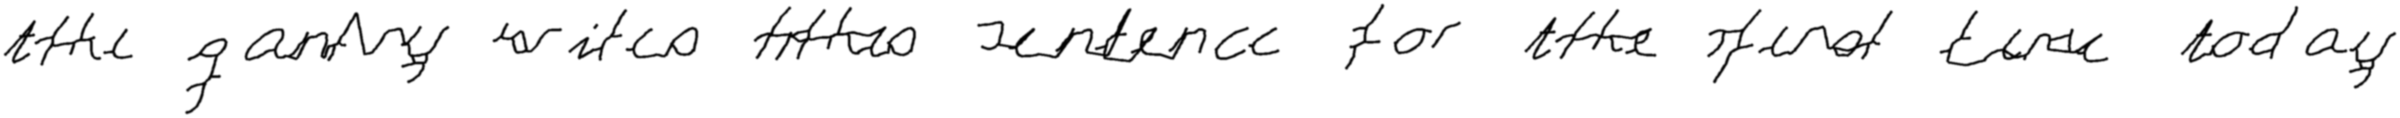
\includegraphics[width=0.95\linewidth]{Figures/w3_synth_153.png}
\caption{Synthesised line for writer 150 (upper, printed hand, read back with three small errors) and writer 153 (lower, joined hand, read back with several letter errors), one seed and candidate each, rendered from an end-to-end run.}
\label{fig:syn-lines}
\end{figure}


A candidate costs one synthesis, one rendering, one recogniser pass and one classifier pass, so the search time is
\begin{equation}
T\approx N\,(T_{\mathrm{syn}}+T_{\mathrm{ren}}+T_{\mathrm{text}}+T_{\mathrm{wid}})+\text{(up to three repair candidates)},
\label{eq:syn-cost}
\end{equation}
each network pass being about $4\times10^9$ multiply--accumulate operations (Equation~\ref{eq:rec-macs}, Table~\ref{tab:wid-layers}).
Table~\ref{tab:syn-cost} resolves Equation~\ref{eq:syn-cost} into its terms on the development laptop, and the result decides where any optimisation must go: synthesis costs 11 to 16\,ms per candidate against 0.5 to 4\,s for the two judges, so the search is entirely judge-bound, and within the judges the dominant cost is thinning the full-resolution render rather than either network.

\begin{table}[!htbp]
\centering
\fontsize{8}{9.6}\selectfont
\setlength{\tabcolsep}{4pt}
\begin{tabularx}{\linewidth}{|X|c|c|c|}
\hline
\textbf{Quantity (56-character sentence)} & \textbf{Writer 150} & \textbf{Writer 153} & \textbf{Writer 551} \\
\hline
Render size (pixels) & $3585\times225$ & $5508\times207$ & $7876\times277$ \\
Synthesis of one candidate (ms) & 11 & 13 & 16 \\
Rendering (ms) & 20 & 27 & 56 \\
Text recogniser (s) & 0.50 & 0.49 & 0.74 \\
Writer classifier incl.\ stroke normalisation (s) & 1.03 & 1.65 & 3.74 \\
Complete search, $N=14$, with repair attempts (s) & 23 & 37 & 137 \\
\hline
\end{tabularx}
\caption{Indicative cost of the search on the development laptop (single profiling run, unknown background load, jitter 0.5); times on the single-board computer were not recorded. The spread across the three writers follows the render width, which follows the writer's own letter size and spacing, so the cost of a search is set by the hand being imitated and not only by $N$.}
\label{tab:syn-cost}
\end{table}

Were the candidate scores independent with distribution function $F$, then $\Pr[\max_kS_k\le\tau]=F(\tau)^N$ and the gain from raising $N$ would grow roughly logarithmically, which is the usual order-statistics argument for a best-of-$N$ scheme.
The seeds share one profile, so independence is only approximate and no per-$N$ curve was kept; the measured values at $N=6$ and $N=14$ in Table~\ref{tab:syn-evid} are consistent with a diminishing return but do not establish its form.

\subsubsection{Alternatives considered}

Four families of handwriting synthesiser were weighed against the glyph library actually built. Table~\ref{tab:syn-alt} sets them against the three quantities that decided the choice for this project: how much data per writer each needs, what it costs per line on hardware with no accelerator, and whether size, slant and spacing can be set as explicit numbers, which requirement R1 needs because the style profile is the deliverable.

\begin{table}[!htbp]
\centering
\fontsize{8}{9.6}\selectfont
\setlength{\tabcolsep}{3.5pt}
\renewcommand{\arraystretch}{1.05}
\begin{tabularx}{\linewidth}{|p{2.6cm}|p{2.3cm}|p{1.9cm}|p{1.6cm}|X|}
\hline
\textbf{Approach} & \textbf{Data needed per writer} & \textbf{Cost per line} & \textbf{Explicit style parameters?} & \textbf{Measured outcome, or why it was not built} \\
\hline
Recurrent generator with attention and a mixture-density stroke output~\cite[p.~1]{graves2013} &
hundreds to thousands of \emph{on-line} pen lines &
not measured &
no &
\textbf{Built and rejected.} A from-scratch version trained on skeleton-derived strokes learned slant, roundness and connectedness but \emph{no legible letters}. Only 47 to 130 scanned lines exist per writer here, and none are on-line. \\
\hline
Adversarial or diffusion generator conditioned on a style exemplar~\cite{kang2020,dai2024} &
less, through pre-training &
\textbf{35 to 45\,s} &
no &
\textbf{Trialled and parked.} Emits a raster needing the same thinning to vectorise, and cannot control size, slant and spacing as numbers. \\
\hline
Exemplar-based synthesis from the writer's own captured letterforms~\cite[p.~26:1]{haines2016} --- \textbf{chosen} &
about \textbf{nine pages}, no training &
\textbf{3 to 8\,s} per line; \textbf{15\,ms} per candidate &
\textbf{yes} &
\textbf{Built and delivered.} Suits a single-board computer with no accelerator. Its one clear weakness is joined hands, whose joins are necessarily lost by the character-cutting of Section~\ref{sec:sty-forced}. \\
\hline
Font-style interpolation from a trained letterform model &
\mustdo{not costed} &
\mustdo{not costed} &
partly &
\mustdo{state whether this was considered, and if so on what grounds it was set aside.} \\
\hline
\end{tabularx}
\caption{Alternatives to the glyph-library synthesiser. Two of the four were implemented far enough to measure; the per-line costs are from the same development laptop as Table~\ref{tab:syn-cost} and are therefore comparable with each other, though not with the single-board computer. The decisive column for this project is the fourth: R1 requires a stored, inspectable style, which a learned generator does not provide.}
\label{tab:syn-alt}
\end{table}

\begin{figure}[htb]
\centering
\figmaybe{syn-alt-comparison.png}{width=0.85\linewidth}{The same short sentence in the same writer's style, rendered four ways and stacked: the writer's real handwriting, the glyph-library synthesis delivered, the rejected recurrent generator's output, and one trialled diffusion sample. The point to show is that the recurrent output carries the slant and roundness but no readable letters, while the glyph library is legible but loses the joins.}
\caption{The same sentence rendered by the writer's own hand and by three of the four approaches of Table~\ref{tab:syn-alt}, showing what each preserves and what each loses.}
\label{fig:syn-alt-comparison}
\end{figure}

\subsubsection{Known faults and limitations}
\label{sec:syn-limits}

\begin{enumerate}\setlength{\itemsep}{0pt}\setlength{\parskip}{0pt}
\item \emph{The legibility mechanism is inert as submitted}, because \texttt{legibilityLambda} is absent from all thirteen stored profiles and defaults to zero, so $\lambda=0$ on the live path: only the unconditional substitutions at $d\ge0.55$ fire, and every $\lambda$-dependent figure above describes a tuned configuration that is not what the delivered profiles currently run.
\item Every figure after the search is introduced is the opinion of the very networks that selected the output: the search loads the same weight files as the measurement, so the values show the pipeline can satisfy its two judges, not that an independent reader would agree.
\item $\lambda$, the anchor threshold and $N$ were tuned on the same sentences Section~\ref{sec:results} measures, and the style calibration of Section~\ref{sec:syn-glyph} measures both sides with the same estimator, so its agreement is partly self-fulfilling.
\item Writers 151 and 552, the two most joined hands, reach only 53 and 56\,\% character accuracy through G-code against about 84\,\% for the other eleven, the clearest limitation of the exemplar approach and a direct consequence of the cutting problem of Section~\ref{sec:sty-forced}.
\item Cutting a joined line destroys how a letter changes shape with its neighbours, which is the underlying reason writers 151 and 551 are reproduced least legibly.
\end{enumerate}

\mustdo{page locators outstanding in this subsection. The sources \texttt{douglas1973, teikari2016, vinciarelli2001, viterbi1967, zhang1984} are each cited here without a page or numbered element. Open each one, find the claim it is cited for, and add the locator in the form \texttt{{\textbackslash}cite[p.~N]\{key\}}, following the rule of \texttt{REFERENCE\_AUDIT.md}: a locator is written only after the source has been read and the claim found, never inferred from a page range or a search snippet.}
